% --------------------------------------------------------------
% This is all preamble stuff that you don't have to worry about.
% Head down to where it says "Start here"
% --------------------------------------------------------------
 
\documentclass[12pt]{article}
 
\usepackage[margin=1in]{geometry} 
\usepackage{amsmath,amsthm,amssymb}
\usepackage{graphicx}

\newcommand{\N}{\mathbb{N}}
\newcommand{\Z}{\mathbb{Z}}
 
\newenvironment{theorem}[2][Theorem]{\begin{trivlist}
\item[\hskip \labelsep {\bfseries #1}\hskip \labelsep {\bfseries #2.}]}{\end{trivlist}}
\newenvironment{lemma}[2][Lemma]{\begin{trivlist}
\item[\hskip \labelsep {\bfseries #1}\hskip \labelsep {\bfseries #2.}]}{\end{trivlist}}
\newenvironment{exercise}[2][Exercise]{\begin{trivlist}
\item[\hskip \labelsep {\bfseries #1}\hskip \labelsep {\bfseries #2.}]}{\end{trivlist}}
\newenvironment{problem}[2][Problem]{\begin{trivlist}
\item[\hskip \labelsep {\bfseries #1}\hskip \labelsep {\bfseries #2.}]}{\end{trivlist}}
\newenvironment{question}[2][Question]{\begin{trivlist}
\item[\hskip \labelsep {\bfseries #1}\hskip \labelsep {\bfseries #2.}]}{\end{trivlist}}
\newenvironment{corollary}[2][Corollary]{\begin{trivlist}
\item[\hskip \labelsep {\bfseries #1}\hskip \labelsep {\bfseries #2.}]}{\end{trivlist}}
\newenvironment{solution}
  {\begin{proof}[Solution]\renewcommand{\qedsymbol}{}}
  {\end{proof}}

\usepackage{listings}
\usepackage{color}
\usepackage{url}

\definecolor{mygreen}{rgb}{0,0.6,0}
\definecolor{mygray}{rgb}{0.5,0.5,0.5}
\definecolor{mymauve}{rgb}{0.58,0,0.82}

\lstset{ %
  backgroundcolor=\color{white},   % choose the background color; you must add \usepackage{color} or \usepackage{xcolor}
  basicstyle=\footnotesize,        % the size of the fonts that are used for the code
  breakatwhitespace=false,         % sets if automatic breaks should only happen at whitespace
  breaklines=true,                 % sets automatic line breaking
  captionpos=b,                    % sets the caption-position to bottom
  commentstyle=\color{mygreen},    % comment style
  deletekeywords={...},            % if you want to delete keywords from the given language
  escapeinside={\%*}{*)},          % if you want to add LaTeX within your code
  extendedchars=true,              % lets you use non-ASCII characters; for 8-bits encodings only, does not work with UTF-8
  frame=single,                    % adds a frame around the code
  keepspaces=true,                 % keeps spaces in text, useful for keeping indentation of code (possibly needs columns=flexible)
  keywordstyle=\color{blue},       % keyword style
  language=c++,                 % the language of the code
  morekeywords={*,...},            % if you want to add more keywords to the set
  numbers=left,                    % where to put the line-numbers; possible values are (none, left, right)
  numbersep=5pt,                   % how far the line-numbers are from the code
  numberstyle=\tiny\color{mygray}, % the style that is used for the line-numbers
  rulecolor=\color{black},         % if not set, the frame-color may be changed on line-breaks within not-black text (e.g. comments (green here))
  showspaces=false,                % show spaces everywhere adding particular underscores; it overrides 'showstringspaces'
  showstringspaces=false,          % underline spaces within strings only
  showtabs=false,                  % show tabs within strings adding particular underscores
  stepnumber=0,                    % the step between two line-numbers. If it's 1, each line will be numbered
  stringstyle=\color{mymauve},     % string literal style
  tabsize=2,                       % sets default tabsize to 2 spaces
  title=\lstname                   % show the filename of files included with \lstinputlisting; also try caption instead of title
}


\begin{document}



 
% --------------------------------------------------------------
%                         Start here
% --------------------------------------------------------------
 
\title{Ray Tracer}%replace X with the appropriate number
\author{Maksim Levental\\ %replace with your name
CAP 4730} %if necessary, replace with your course title
 
\maketitle
\newpage
\tableofcontents
\newpage
\begin{abstract}

Ray tracing is a basic method of rendering a three dimensional scene on a viewing plane. Light rays are modeled as vectors with origin at every pixel in viewing plane and direction. These rays are then tested for intersection against objects in the scene. Intersection tests are unique to each figure type. Shading is effected by comparing various dot products between the normal to the surface of the object, the intersection ray, and the light source vector. Ambient light is a global constant. Efficiency and numerical stability is poor.

\end{abstract}

\section{Introduction}

Ray tracing is a way to image objects in a virtual scene. That is to say if one wishes to represent a collection of 3D objects, for each of which one has an implicit representation, on a 2D image plane. Its efficacy relies on the idea that light can be modeled by ray/geometric optics. The basic idea is to treat every pixel in the image plane as a source for such an optical ray and then to simulate the effects of that ray's interaction with objects in the virtual scene.

\subsection{Intersection}

The simplest interaction the ray could have with an object is that it might intersect that object. Testing for such an intersection requires having an implicit representation for that object. To be precise a ray has the parametric vector representation 

$$ \vec{f}(t) = \vec{P} + t \vec{D} $$

\noindent where $\vec{P}$ is the origin of the ray, $\vec{D}$ is the direction of the ray, and $\vec{f}$ ranges through all the vectors to points on the line as $t$ ranges from $0$ to $+\infty$. Implicit representations of objects in the scene are a collection ${g(\vec{x})}$\footnote{We interpret $g$ as any process for testing whether $\vec{x}$ is a ``root''.} such that 
$$ g(\vec{x}) = 0 $$
for all $\vec{x}$ that correspond to points on that object. 

\subsubsection{Sphere}

For the case of a sphere \cite{wiki:Ray_tracing_(graphics)} with center $\vec{c}$ and radius $r$

$$g(\vec{x}) = g(\vec{f}(t)) = \left\Vert\vec{P}+t\vec{D}-\vec{c}\right\Vert^{2}-r^2 = 0.$$
Equivalently define $\vec{v} = \vec{P} - \vec{c}$ then if 

$$t =-(\vec{v}\cdot\vec{D})\pm\sqrt{(\vec{v}\cdot\vec{D})^2-(\vec{v}^2-r^2)} $$
is real the ray intersects the sphere.

\subsubsection{Triangle}
\label{subsec:triangle}
For the case of a triangle the intersection test is more complex \cite{doi:10.1080/10867651.2003.10487593}. Define for each ray $r$ 

$$\pi_r = (\vec{D},\vec{D} \times \vec{P}) \equiv (\vec{U}_r,\vec{V}_r)$$
and

$$\pi_i \odot \pi_j = \vec{U}_i \cdot \vec{V}_j + \vec{U}_j \cdot \vec{V}_i.$$
For each edge $e_i$ of the triangle assert $\pi_{e_i}$. Then the ray intersects the triangle iff

$$ \pi_r \odot \pi_{e_i} \geq 0 ~ \forall i~ \text{and}~ \exists j \: \pi_r \odot \pi_{e_j} \neq 0 $$
\begin{center}or\end{center}
$$ \pi_r \odot \pi_{e_i} \leq 0 ~ \forall i~ \text{and}~ \exists j \: \pi_r \odot \pi_{e_j} \neq 0. $$
\subsection{Shading}

A slightly more complex interaction that a ray could have with an object is specular reflection/refraction. If there is a light source (ambient light is discussed blow) then the degree to which the ray is refracted can be used to appropriately ``shade'' the surface using the Phong lighting model. 

There are three components to the light cast on the object: ambient, which is just a global constant energy added to all points, diffuse, which is a function of the normal to the surface and the direction from the point to the light source, and specular, which is a function of the point of view of the virtual camera and the direction of the light source. 

\subsubsection{Diffuse}

Diffuse light is calculated as
 
$$I\, k_d\, \text{max}(0,\vec{n}\cdot\vec{v}_l)$$ 
where $I$ is a global illumination constant, $k_d$ is the diffusion constant (to modulate how potent the diffuse lighting is), $\vec{n}$ is the normal to the surface, and $\vec{v}_l$ is the direction to the light source. Taking the maximum of $0$ and $\vec{n}\cdot\vec{v}_l$ is done because the normal might be in the opposite direction of the source of light, if for example a point on a hidden section of the object is intersected by the viewing ray.

\subsubsection{Specular}

Specular lighting is typically computed as 

$$I\, k_d\, \text{max}(0,\vec{v}_r\cdot(2(\vec{n}\cdot\vec{v}_l)-\vec{v}_l))^n$$
but this is too computationally inefficient so the reflection ray, $2(\vec{n}\cdot\vec{v}_l)-\vec{v}_l)$ is approximated by the bisector vector of $\vec{l}$ and $\vec{r}$

$$\vec{v}_H = \text{bisector}(\vec{v}_l,\vec{r}) = \frac{(\vec{v}_l + \vec{v}_r)}{\left\Vert \vec{v}_l + \vec{v}_r \right\Vert} $$
Hence the specular shading gradient is computed as 

$$I\, k_s\, \text{max}(0,\vec{n}\cdot\vec{v}_H)^n$$

\subsubsection{Lighting}

Total lighting applied to the surface of the object is then

$$k_a I_a + I_w\Big(k_d\, \text{max}(0,\vec{n}\cdot\vec{v}_l) + k_s\, \text{max}(0,\vec{n}\cdot\vec{v}_H)^n\Big)$$
where $k_a$ and $I_a$ are constants ambient lighting constant that apply a warm hue to the scene. 
\section{Implementation}

The ray tracer algorithm is implemented in C++ using the Boost library uBLAS \cite{ublas} for the linear algebra components and the freeglut OpenGL api to actually draw the window.

\subsection{\texttt{surfaces.h}}

This defines the classes for the two main surface types ``traced'' by the ray tracer, spheres and triangles. Each class derives from the base class \texttt{surface}, which defines 3 pure virtual methods (\texttt{intersection\_test}, \texttt{unit\_normal}, \texttt{test}) that each subclass should implement, and the base member that all subclasses share \texttt{color}, which is of type \texttt{GLubyte}, a typedef from the freeglut library for \texttt{char}. \texttt{intersection\_test} takes as arguments the ray origin and the ray direction and returns the distance of the intersection point from the viewing plane or -1 in case there is no intersection. 

\texttt{surfaces.h} also defines typedefs for commonly used vectors from the uBLAS library, global constants for the light source direction, the viewing plane pixel array (\texttt{checkImage}), and shading constants. Finally \texttt{surfaces.h} defines 3 helper functions: \texttt{rotate\_viewing\_angle} is necessary for effecting rotations of the camera perspective, \texttt{cross\_product} is the cross product in 3 dimensions (because that is absent from uBLAS), and \texttt{loadbar} is a loading bar that shows progress of rendering in the console.

\subsubsection{\texttt{sphere} class}

The constructor takes as arguments a \texttt{GLubyte[3]} RGB color, a \texttt{dbl\_vec} center, and a radius.

\subsubsection{\texttt{triangle} class}

The constructor takes as arguments a \texttt{GLubyte[3]} RGB color, and 3 \texttt{dbl\_vec} vertices in counter-clockwise order. That is to say the orientation of the triangle is right-handed, so if the triangle vertices passed are $(0,1,0)$,$(0,0,0)$, and $(1,0,0)$ then the normal would be in the $\vec{k}$ direction. This is important for the shading algorithm.



Note \texttt{plucker\_edgeXY[2]} in the \texttt{triangle} class is $\pi_{e_i}$ discussed in \ref{subsec:triangle} . 

\subsection{\texttt{ray\_tracer.cpp}}

This implements the actual ray tracing algorithm.
\subsubsection{\texttt{makeCheckImage}}

For every pixel in the viewport, each of which corresponds to the entries in the \texttt{checkImage} array defined in \texttt{surfaces.h}, a \texttt{long\_double\_vec} is created. Then for each object in the scene, pointers to which are all stored in the global \texttt{std::vector<surface*>} container, the intersection test for that class is run. If there is in fact intersection then that object is stored in a \texttt{std::map<double,surface*>} container with key equal to the distance from the viewing plane. This is so that if the ray intersects many objects the one with the smallest distance (key) will be the first element in the \texttt{map}.

If any objects are intersected then the shader method of the nearest one (first element in \texttt{map} as mentioned above) is called to color the corresponding entry in \texttt{checkImage}. Otherwise \texttt{checkImage} is set to black.

A red bounding box is drawn around the viewing plane as well.

\subsubsection{\texttt{keyPressed}}
\textbf{Rotations of the camera perspective upon key press are implemented. Pressing \texttt{d} on the keyboard rotates $10$ degrees counter-clockwise around the $z$-axis and pressing \texttt{a} undoes this rotation. Pressing \texttt{w} on the keyboard rotates $10$ degrees counter-clockwise around the $y$-axis and pressing \texttt{s} undoes this.}
\subsubsection{\texttt{main}}

Objects are instantiated and added to the \texttt{std::vector<surface*> surfaces} container. \texttt{int\_vec push} can be used to translated objects by adding to either the center, in the case of a \texttt{sphere}, or to all vertices, in the case of a \texttt{triangle}.

\section{Testing}

\subsection{Only ambient}
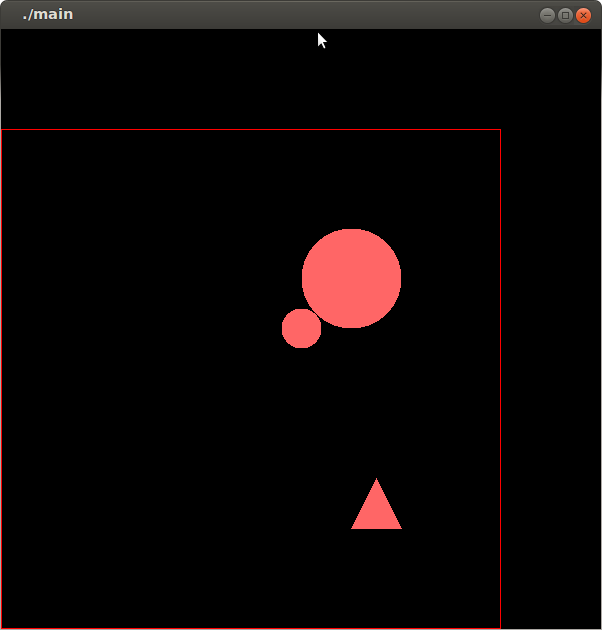
\includegraphics[scale=.75]{ambient.png}
\subsection{Only diffuse}
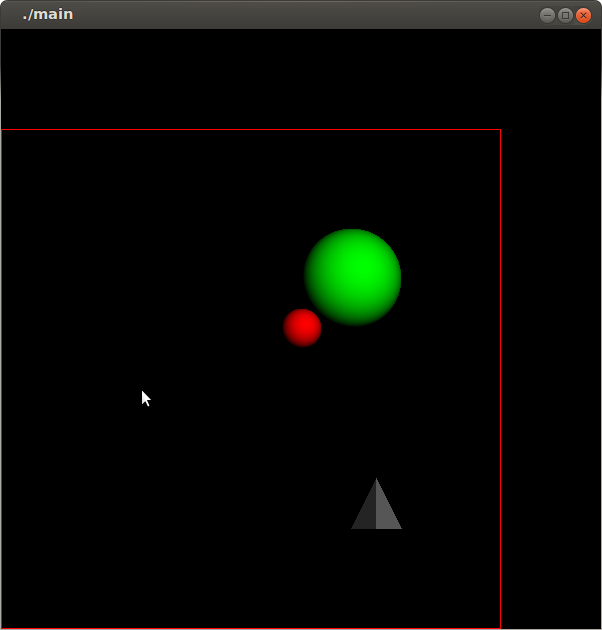
\includegraphics[scale=.75]{diffuse.png}
\subsection{Only specular}
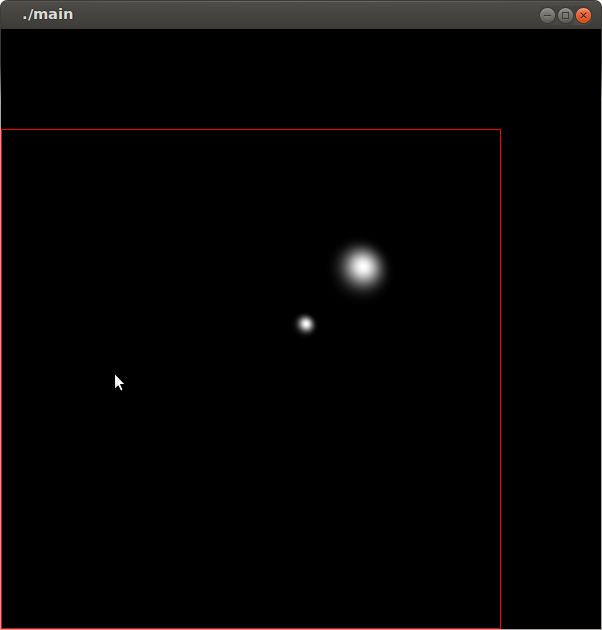
\includegraphics[scale=.75]{specular.png}
\subsection{Specular and diffuse}
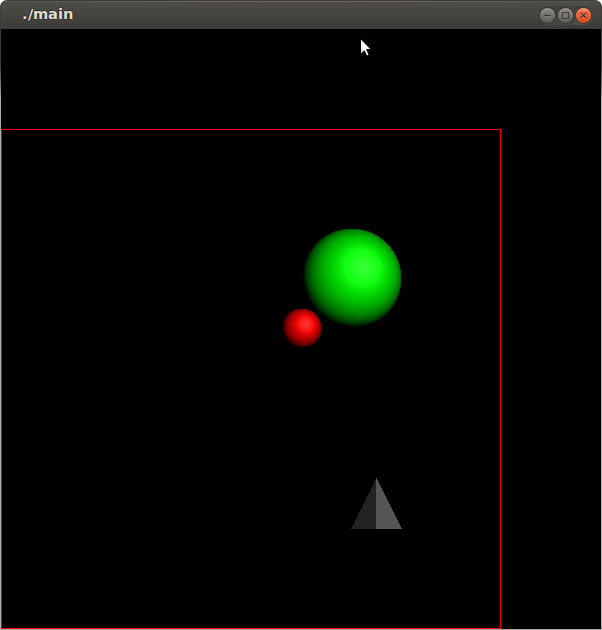
\includegraphics[scale=.75]{speculardiffuse.png}
\subsection{Final}
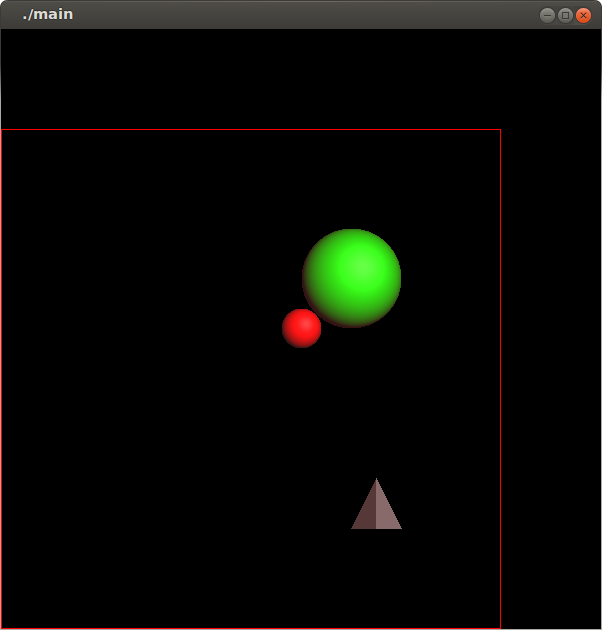
\includegraphics[scale=.75]{final.png}


\section{Conclusion}

While ray tracing is a simple algorithm to implement it is not numerically stable. For example when implementing rotations it was necessary to change the intersection test in the \texttt{triangle} class. \texttt{double diff} had to be introduced because the naive check checked whether 

\begin{lstlisting}
abs(norm_plucker) == ( abs(sidetestAB)+abs(sidetestBC)+abs(sidetestCA) ) 
\end{lstlisting}
but this ceased to work because of accumulated floating point error. Hence checking that they were within an interval of each other. 

Furthermore testing rays emanating from every pixel in the viewing plane is very inefficient because most of the scene is empty. \textbf{The addition of the tetrahedron to the scene did noticably slow rendering but that's simply because said tetrahedron is small. Given the complexity of the intersection test for the \texttt{triangle} class it is obvious that were the tetrahedron bigger it would greatly slow the rendering.}
% --------------------------------------------------------------
%     You don't have to mess with anything below this line.
% --------------------------------------------------------------
\bibliographystyle{plain}
\bibliography{citations}

\end{document}
\begin{align*}
\sum_{i=1}^{k+1}i & = \left(\sum_{i=1}^{k}i\right) +(k+1)\\ 
& = \frac{k(k+1)}{2}+k+1 & (\text{by inductive hypothesis})\\
& = \frac{k(k+1)+2(k+1)}{2}\\
& = \frac{(k+1)(k+2)}{2}\\
& = \frac{(k+1)((k+1)+1)}{2}.
\end{align*}
